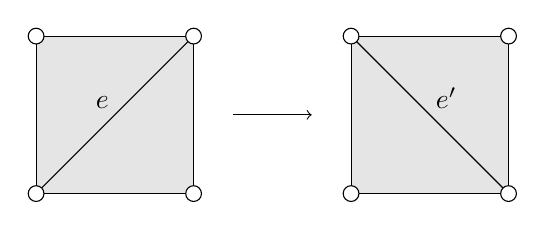
\begin{tikzpicture}[every node/.style={inner sep=2pt}]
\coordinate (A) at (0,0);
\coordinate (B) at (2,0);
\coordinate (C) at (2,2);
\coordinate (D) at (0,2);
\draw[fill=gray!20] (A) rectangle (C);
\draw (C) to node[above left]{$e$} (A);
\draw[fill=white] (A)circle(0.1) (B)circle(0.1) (C)circle(0.1) (D)circle(0.1);

\draw[->] (2.5,1) -- (3.5,1);

\begin{scope}[xshift=4cm]
\coordinate (A) at (0,0);
\coordinate (B) at (2,0);
\coordinate (C) at (2,2);
\coordinate (D) at (0,2);
\draw[fill=gray!20] (A) rectangle (C);
\draw (B) to node[above right]{$e'$} (D);
\draw[fill=white] (A)circle(0.1) (B)circle(0.1) (C)circle(0.1) (D)circle(0.1);
\end{scope}
\end{tikzpicture}